\documentclass[12pt]{article}
\usepackage{sbc-template}
\usepackage{graphicx,url}
\usepackage[brazil]{babel}
\usepackage[utf8]{inputenc}
\usepackage{todonotes}
\usepackage{graphicx}
\usepackage{placeins}
\usepackage{indentfirst}


\sloppy

\title{Transmissão de Vídeo em Tempo Real em Redes AD HOC}

\author{Anderson Andrei\inst{1}, Patrick Abrahão\inst{1}, Roger Immich\inst{2}, Alfredo Goldman\inst{1}}
\address{Instituto de Matemática e Estatística \\ 
Universidade de São Paulo(USP)
  \nextinstitute Instituto de Computação \\ 
  Universidade Estadual de Campinas (UNICAMP)
  %
  %
  % Roger: hack para deixar os emails em 2 linhas próximas... tem alguma forma melhor melhor?
  %
  %
  \email{\{anderson.andrei.silva, patrick.menani\}@usp.br,}\vspace{-0.4cm}
  \email{roger@lrc.ic.unicamp.br, gold@ime.usp.br}
} 


\begin{document} 

\maketitle

\begin{abstract}
In the next few years is expected a considerable growth of video transmission in wireless networks, this is especially true considering mobile devices. In the light of this, the main goal of this work is to perform a quantitative and qualitative analysis of the real-time video transmission between mobile devices. This is important to better understand all the details involved in this process.
In order to do that, several methods of package transmission of live video stream were analyzed. Using a network simulator OMNeT++ and the INET Framework, these methods were assessed and classified according to their qualities and scalability. A comparison between the protocols TCP, UDP, and the transmission technique DASH is also presented. So, we did analysis with the metrics of delay in the delivery of the packages, among of KiB received by the receiver host and the package loss and required rate.
\end{abstract}
     
\begin{resumo}
Nos próximos anos é esperado um grande crescimento da transmissão de vídeos em redes sem fio, especialmente em dispositivos móveis.
Baseando-se nesta crescente demanda, o principal objetivo deste trabalho é o de realizar uma análise quantitativa e qualitativa sobre a transmissão de vídeo em tempo real entre dispositivos móveis. Com isto, é esperado obter-se um melhor entendimento de alguns aspectos ligados à transmissão de dados. Para tal, foram analisadas algumas formas de transmissão de pacotes na rede para vídeo ao vivo. Através de simulações foi possível realizar comparações entre as diversas formas afim de classificá-las quanto sua qualidade e a escalabilidade na rede. As comparações foram feitas entre os protocolos TCP, UDP e a técnica de transmissão DASH através de simulações feitas no OMNeT++ e o INET Framework. Assim, fizemos análises com as métricas de \textit{delay} na entrega dos pacotes, quantidade total de \textit{KiB} recebidos pelo \textit{host} destino e a taxa de pacote recebidos e requisitados.
\end{resumo}

% tirei o pagebreak
%\pagebreak{}
\section{Introdução} \label{sec:introducao}
	
    Nos últimos anos houve um grande aumento na utilização de aplicações de vídeo. Estas aplicações estão presentes nas redes sociais, serviços de vídeo sob demanda e até em jogos interativos. Para aumentar ainda mais a demanda, cada vez mais são produzidos mais e melhores dispositivos móveis~\cite{Adobe2017}, colocando um grande poder de processamento nas mãos dos usuários. Isto permite o fácil acesso à produção, consumo e disponibilização de conteúdos multimídia. Todas as facilidades levam a um considerável aumento no tráfego de rede. Somente para citar um exemplo, de acordo com a Cisco, até 2021 o tráfego global de toda a Internet deverá ser 127 vezes maior do que foi em 2005. De todo este tráfego, é esperado que a transmissão de vídeo represente mais de 82\% do total~\cite{Cisco2017}. Levando-se em consideração este grande crescimento na demanda pela transmissão de vídeo, este trabalho visa estudar a transmissão de dados em tempo real em redes veiculares tendo como maior motivação o cenário de veículos autônomos. Redes veiculares tem apresentado atualmente vantagens como controle eficiente de tráfego, maior segurança e possibilidade de desenvolvimento de novos recursos~\cite{Yi:2015:SFC:2757384.2757397}. Esse é um ambiente composto por uma estrutura capaz de fornecer dados para veículos que trafegam em uma determinada área, e outra estrutura que configura o conjunto de veículos que utilizarão o serviço.
    
	Dada a complexidade de trabalhar com esse ambiente, em um primeiro momento, reduzimos nosso cenário de estudo para uma rede \textit{AD-HOC}. Estas redes são compostas por dispositivos móveis que não necessitam de uma infra-estrutura de rede por trás e possuem movimentação, tendo assim cenários dinâmicos. Assim sendo, vamos estudar pontos de qualidade de serviço e de experiência do usuário para a transmissão de vídeo em tempo real em redes AD-HOC. Vamos fazer comparações entre dois protocolos de transmissão, \textit{TCP} e \textit{UDP}, e o \textit{DASH}, uma técnica aplicada no primeiro deles que permite a mudança da qualidade da transmissão de vídeo de acordo com a qualidade da rede. Utilizaremos o simulador de redes \textit{OMNeT++}~\cite{omnet} com a extensão\textit{ INET Framework}~\cite{inet} que nos possibilita trabalhar também com cenários móveis e redes \textit{wireless}. A partir dessas simulações vamos analisar requisição e perda de pacote, o \textit{delay} na entrega deles e a quantidade total de \textit{KiB} recebidos pelo dispositivo destino para analisar qual deles pode ser melhor em determinados cenários.
    Nesse trabalho são apresentados alguns conceitos sobre redes \textit{AD-HOC}, transmissão de vídeo em tempo real, a técnica de transmissão \textit{DASH} e os critérios de avaliação que serão utilizados na análise. Também serão apresentados alguns trabalhos relacionados, os dados obtidos e suas respectivas análises. Por fim, será apresentada a conclusão e trabalhos futuros.
    
\section{Conceitos fundamentais} \label{sec:conceitos}

	A transmissão de vídeos em tempo real é algo complexo que demanda o estudo da estrutura da rede que será utilizada, das ferramentas responsáveis pela transmissão do vídeo, sua qualidade e integridade, entre diversos outros conceitos~\cite{Immich2017a}. Assim sendo, serão apresentados alguns conceitos fundamentais utilizados no desenvolvimento deste trabalho.

\subsection{Redes AD HOC}
    Uma rede móvel AD HOC, do inglês \textit{MANET} e também conhecida como \textit{WANET (Wireless Ad Hoc Network)} é uma rede composta por um conjuntos de dispositivos wireless que não precisam, necessariamente, de uma infra estrutura de rede pré existente. É uma rede decentralizada e auto organizada onde as comunicações são feitas de forma \textit{multi-hop}, ou seja, partem de um dispositivo fonte para um dispositivo destino sendo transmitidas através de dispositivos que estão localizados entres esses dois. De acordo com a mobilidade de tais dispositivos, estas redes apresentam características altamente dinâmicas, o que dificulta a análise de qualidade de serviço e experiência do usuário final~\cite{Immich2018}.

\subsection{Transmissão de vídeo em tempo real}
	Conforme mencionado anteriormente, serviços de transmissão de vídeos em tempo real tem ganhado espaço nas rotinas diárias em todo o Mundo, e tem sido utilizados com propósitos desde educacionais até de entretenimento. O rápido avanço no consumo desse tipo de serviço é evidente nos últimos anos, particularmente em dispositivos móveis e sem fio~\cite{Adobe2017}. Isso se deve aos avanços tecnológicos de dispositivos que abrangem maior conectividade e a maior adoção de dispositivos \textit{smart}. Muitas companhias tem usado transmissão de vídeo como meio de negócio para aumentar sua produtividade, melhorar a colaboração, reduzir custos e optimizar processos operacionais. Na mesma via, usuários não profissionais tem produzido e compartilhado milhões de vídeos utilizando tais mecanismos e dispositivos~\cite{Cisco2017}.

\subsection{Técnica de transmissão DASH}
	Essa é uma técnica aplicada no protocolo TCP e permite ao cliente redimensionar e optar pelo melhor \textit{bitrate}. Dependendo das limitações de recursos oferece uma maneira eficiente de proporcionar a melhor qualidade possível para o usuário. Ou seja, essa técnica faz com que a qualidade do vídeo diminua caso a qualidade da rede seja baixa ou fique assim por algum motivo. Da mesma forma, se a qualidade da rede é alta o suficiente, a qualidade do vídeo transmitido será proporcionalmente alto. Logo é mais garantida a transmissão do vídeo em tempo real em maiores circunstancias~\cite{5} .  
%	Os seguintes pontos cobrem suas características mais importantes para o nosso estudo :
   
%  \begin{itemize}
%  \item "Deployment on Standard HTTP Servers", facilita a implementação em servidores comuns, sem um gasto adicional para a implementação;
%  \item "Fast Channel Switching", é diretamente relacionado ao tamanho dos pedaços em que a mídia é dividida, algumas implementações dividem em tamanhos de 10 segundos, mas o DASH divide em tamanhos de 2 a 4 segundos, facilitando uma rápida troca de qualidade entre os períodos da mídia;
%  \item "Support Multiple CDNs \cite{6} in Parallel", fornece uma forma de sinalização nativa para se obter conteúdo em paralelo de diversas fontes, isso permite ao cliente escolher a melhor fonte;
%  \item "HTML5 Support", utilizando as extensões de vídeo do HTML5 é possível utilizar a função nativa de reprodução dos buscadores atuais;
%  \item "Agnostic to Video Codecs and Audio Codecs \cite{7} ", permite trabalhar com diversos codificadores de vídeo e áudio, permite a escolha daquele que parecer melhor à aplicação;
%  \item "Definition of Quality Metrics":, permite e estabelece para o cliente métricas para avaliações de aspectos da qualidade do serviço;
%  \item "Client Logging and Reporting", oferece uma interface padrão de reporte de qualidade de serviço;
%  \item "Client Failover", oferece um mecanismo de checagem de falha das CDNs, permitindo o cliente baixar um mesmo segmento de diversas fontes, evitando perdas;
%  \item "Multiple Video Views", permite ao usuário optar por ângulos diferentes de visualização caso seja oferecido pelo provedor, isso é muito usado em transmissões ao vivo de fórmula 1 e pode ser facilmente utilizado na nossa aplicação em transmissões esportivas interativas num futuro;
%  \end{itemize} 
  
\subsection{Critérios de comparação}
    Para analisarmos os dados obtidos utilizaremos como critério de comparação requisição e perda de pacotes, quantidade de \textit{KiB} recebidos pelo \textit{host destino} e o \textit{delay} na entrega deles. O primeiro é o número de pacotes requisitados e taxa de perda deles dentro da trajetória até seu destino final. O segundo se trata da quantidade de informação de vídeo recebido pelo cliente e o último é o quanto de atraso ocorreu na entrega dos pacotes.

\section{Trabalhos relacionados} \label{sec:trabalhos}
	Esse trabalho está inserido no projeto INCT da Internet do Futuro para Cidades Inteligentes : \textit{"Improving fog computing techniques to allow a better quality of experience in vehicular networks"}, e no mesmo contexto da pesquisa apresentada foram encontramos diversos trabalhos relacionados. Isto demonstra que o trabalho desenvolvido está inserido em um assunto importante e com um grande potencial de crescimento.
    
    O aumento do uso de \textit{cloud computing} requer atenção por ainda envolver vários pontos não resolvidos como latência não confiável, falta de mobilidade e pontos de localização para disponibilização da rede. \textit{Fog computing} ou \textit{edge computing} aparece então nesse cenário provendo recursos e serviços maleáveis para os usuários finais através da borda da rede, enquanto, em conjunto, a \textit{cloud computing} passa a ser responsável pela rede central, solucionando assim o problema de falta de mobilidade. Tratando a questão da latência, a \textit{fog computing} fornece dinamismo e maior confiabilidade de conexão. Por outro lado, para melhor aproveitar recursos como capacidade e banda, é preciso analisar como e onde pré armazenar dados para tornar mais prática a computação dos dados e esse tem sido um dos desafios~\cite{Yi:2015:SFC:2757384.2757397}. Nesse mesmo segmento são estudadas decisões quanto a troca de informação utilizando máquinas virtuais, análises do gerenciamento de recursos e da comunicação entre servidor e veículos ao longo de estradas~\cite{Yao:2015:MEV:2915680.2915702}. Essa comunicação por parte do servidor e do veículo pode falhar em algum momento ou até não alcançar um determinado veículo e então é desejado que o mesmo possa se comunicar com outros que tenham esta conexão estabelecida, mantendo assim o fluxo de dados ao longo de um percurso~\cite{Simula.simula.2416}.
    
    Além disso, também são estudadas configurações e composições de vídeos. Esses são formados por \textit{frames} e utilizados de formas diferentes dependendo do tipo de \textit{codec} utilizado. Esses \textit{frames} possuem diferenças em suas composições podendo ser classificados em três tipos diferentes de prioridades e ainda se relacionam dependentemente entre si. Logo, ocasionalmente a perda de um \textit{frame} em específico pode afetar um longo trecho de vídeo, o que é diretamente perceptível ao usuário, e então é um sério problema de qualidade de experiência. Por isso são estudados e desenvolvidos métodos de como tratar e evitar tais problemas, também aplicados em transmissão de vídeo em tempo real em redes AD-HOC. Assim sendo, conceitos como esses, técnicas para seu funcionamento e as especificidades da rede que permite esse uso tem sido foco de estudos~\cite{Immich2018}.
    
\section{Cenários experimentais} \label{sec:cenariosexp}

	Nessa primeira abordagem será simulada a transmissão de vídeo em tempo real em uma rede AD-HOC. Esta rede será composta por vários dispositivos móveis, chamados de \textit{hosts}. Todos eles possuem as mesmas características, porém variam entre três configurações distintas, são elas: emissor, receptor e intermediador. O primeiro é aquele que envia os dados, o segundo é quem deve recebê-los e o último é aquele que repassa os dados construindo um caminho ligando o emissor até o receptor. Para o envio de pacotes em uma rede são necessários protocolos que encapsulam as informações antes do envio. Existem diferentes protocolos que atuam de maneiras distintas. Neste trabalho, serão utilizados os protocolos TCP e UDP e ainda a técnica DASH, aplicada em cima do TCP. A utilização do DASH nesse trabalho é uma adaptação da implementação disponível no \textit{GitHub} de Navarro Joaquin~\cite{navarro}.%
    
\subsection{Modelo estudado}
	Os cenários implementados são compostos por um \textit{host} emissor, \textit{hostA}. Um \textit{host} receptor, \textit{hostB}, e $n$ \textit{hosts} intermediadores, $hostR (1,2,3, ... n)$. Os \textit{hosts} $A$ e $B$ terão suas posições iniciais fixadas dentro do cenário, já os \textit{hosts} $R$ serão posicionados aleatoriamente. A quantidade de \textit{hosts} $R$ também será alterada entre as quantidades 50, 100 e 150. Todos os \textit{hosts} se movimentam em duas velocidades, 3 e 6 m/s, gerando diferentes caminhos para o envio dos dados e consequentemente, dinamismo na rede. A área do cenário de testes é de 1000 x 700 m e no total, serão avaliadas 6 variações de cenários distintas, que são, três quantidades diferentes de \textit{hosts} com movimentação lenta e as mesmas três quantidades diferentes de \textit{hosts} com movimentação rápida. A duração do vídeo transmitido nas simulações é de 90s. O tamanho dos pacotes do UDP e TCP foram fixados em 60 KiB, para o DASH colocamos o mais próximo disso como tamanho inicial, já que o mesmo se modifica no decorrer da simulação.%A figura ~\ref{fig:cenario} exemplifica um cenário com 50 \textit{hosts}, apontando quem são os \textit{hosts} A e B.

%\begin{figure}[htpb]
%  \begin{minipage}{\textwidth}
%    \centering
%    \begin{minipage}{.5\textwidth}
%    	\centering
%       	\caption{\textit{Cenário com 50 hosts}}
%        	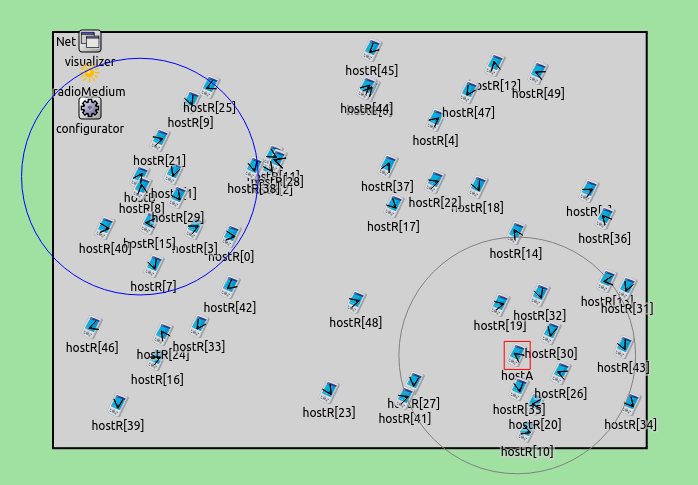
\includegraphics[width=.95\textwidth]{cenario.png}
%    	\label{fig:cenario}
%    \end{minipage}%
%   \end{minipage}
%\end{figure}
%\FloatBarrier

%\subsection{Histogramas} \label{sec:hist}
%%%%%%%%%%%%%%%%% FIGURE : UDP %%%%%%%%5%%%%%%%%%%
%\begin{figure}[h!]
%  \begin{minipage}{\textwidth}
%    %\caption{width=.2\linewidth}
%    \centering
%    \begin{minipage}{.48\textwidth}
%    	\centering
%       	\caption{\textit{UDP350}}
%        	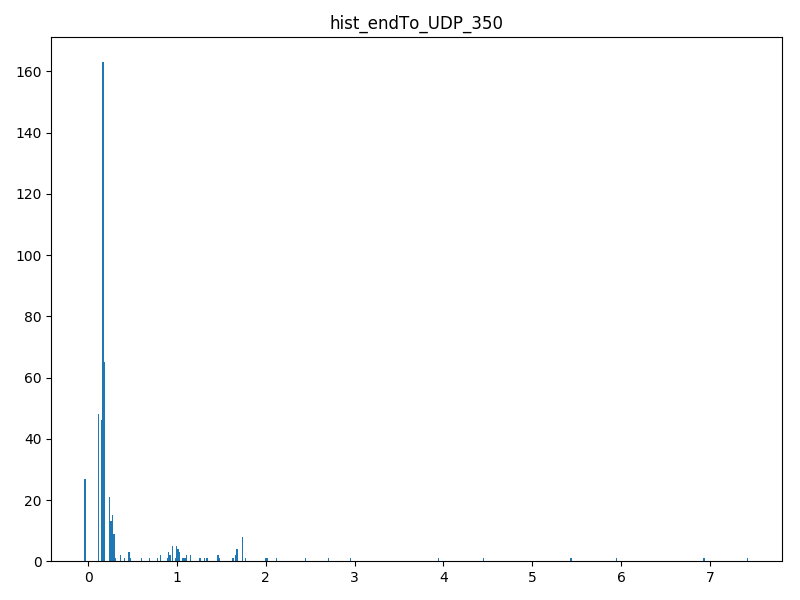
\includegraphics[width=.95\textwidth]{udp350.png}
%    	\label{fig:regions}
%    \end{minipage}%
%    \begin{minipage}{.48\textwidth}
%    	\centering
%        \caption{\textit{UDP 650}}
%        	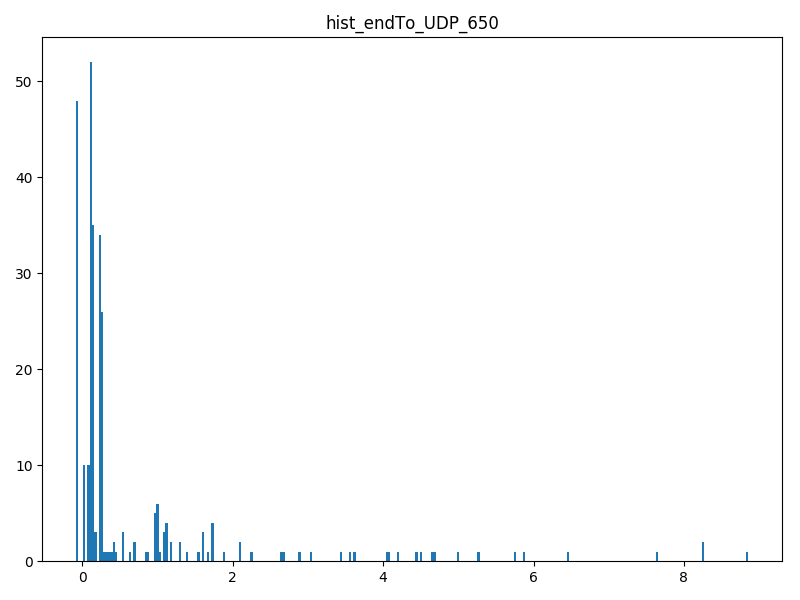
\includegraphics[width=.95\textwidth]{udp650.png}
%    	\label{fig:regions}
%    \end{minipage}
%   \end{minipage}
%\end{figure}
%\FloatBarrier

\section{Análise de performance e resultados} \label{sec:analise}
	Foram executadas 10 simulações para cada modelo de cenário descrito acima nos protocolos TCP, UDP e DASH, sendo então, 60 simulações para cada um deles, totalizando 180 amostras de resultados. A partir desses dados foi obtida a média e alguns desvios padrões para as métricas de \textit{delay}, total de \textit{KiB} recebidos pelo \textit{hostB} e quantidade de pacotes requisitados e sua taxa de perda. Também foram gerados histogramas para o \textit{delay} e estão disponíveis no repositório do projeto~\cite{ic}, seus nomes são compostos por \textit{PROTOCOLO\_(velocidade)(número de \textit{hosts})} e seus dados foram traduzidos em algumas das tabelas que serão exibidas abaixo.
%~\footnote{\url{https://github.com/andersonandrei/VehicularNetworksIC/}}
\subsection{\textit{Delay}}
%	Calculamos o delay na entrega dos pacotes enviados do \textit{hostA} para o \textit{hostB}. A tabela ~\ref{tab:tabledelay}, abaixo, apresenta a média e desvio da simulações dos três protocolos variando também a quantidade de \textit{hosts}.
	A partir da tabela ~\ref{tab:tabledelay} é possível observar que o UDP apresenta valores próximos de zero, variando, nos cenários de velocidade 3 m/s entre 0.41 e 0.6, e nos cenários de 6 m/s entre nan (valor minimamente pequeno) e 2.23. A maior surpresa foi o maior valor ocorrer para a velocidade de 6 m/s com 150 hosts, mas no geral, o UDP se mostrou muito bem em relação a essa métrica. Já o TCP, possui em todos os casos valores maiores que o UDP. Para os cenário de velocidade de 3 m/s varia entre 2.20 e 3.16, melhorando seu rendimento conforme o aumento no número de \textit{hosts}, enquanto, para os cenários com velocidade 6 m/s varia entre 2.77 e 5.07, tendo também seu maior valor no cenário de maior velocidade e maior quantidade de \textit{hosts}. Esses valores podem ser maiores que os do UDP pelo fato dele não fazer verificações, como as de destinatário dos pacotes por exemplo, antes de enviá-los, enquanto o TCP faz. O DASH aumenta um pouco seu intervalo de valores em relação ao TCP, variado entre 3.66 e 5.53  na velocidade de 3 m/s, e 4.98 e 5.84 na velocidade de 6 m/s. O que pode ser percebido é que a variação entre esses valores é menor no caso com maior velocidade, e pode ser assumido que os valores do DASH são um pouco maiores que os do TCP devido a maior quantidade de processos de controle da rede que o DASH faz.
\begin{table}[h!] 
  \centering
  \caption{UDP, TCP, DASH delay}
  \begin{tabular}{c|ccc|ccc}
    \hline
    \multicolumn{1}{c}{} & \multicolumn{3}{c}{Velocity of hosts : 3m/s} & \multicolumn{3}{c}{Velocity of hosts : 6m/s} 			\\ 
    Parameters             & 50 hosts      & 100 hosts     & 150 hosts     &   50 hosts      & 100 hosts     & 150 hosts     		\\ 
    \hline
    \hline
    \multicolumn{7}{c}{\textit{UDP}} \\
    \hline
    \hline
    Mean         & 0.49     & 0.60   & 0.41   &    0.94  & nan    &  2.23  \\
    Stddev       & 0.55    & 0.81   & 0.40   &    1.14  & nan    &  1.67  \\
    \hline
    \hline
    \multicolumn{7}{c}{\textit{TCP}} \\
    \hline
    \hline
    Mean         & 3.16   & 2.91   & 2.20   &    3.83  & 2.77    &  5.07  \\
    Stddev       & 4.96   & 3.59   & 1.90   &    5.91  & 2.81    &  5.13  \\
    \hline
    \hline
    \multicolumn{7}{c}{\textit{DASH}} \\
    \hline
    \hline
      Mean         & 5.53   & 3.82   & 3.66   &    5.84  & 4.98    &  5.55  \\
      Stddev       & 7.56  & 3.65   & 3.12   &    7.44  & 5.84    &  4.97  \\
    \hline
  \end{tabular}
  \label{tab:tabledelay}
\end{table}
\FloatBarrier

	

\subsection{Requisição e Perda de Pacotes} \label{sec:perda}
    A tabela ~\ref{tab:tableperda}, abaixo, apresenta o número de pacotes requisitados e a taxa de perda dos mesmos, com variação na quantidade de \textit{hosts}. A partir dela foi observado que o UDP requisita, em todos os casos, valores próximos de 90 pacotes, e como simulamos a transmissão de 90s de vídeo, apontamos que o UDP consiga transmitir 1s de vídeo por pacote nos cenários simulados. Os resultados mostram uma perda de cerca de 50\% dos pacotes em quase todos os casos, exceto no cenário de 3 m/s com 150 \textit{hosts}, 33.90\%, mas ainda assim é um valor considerado alto pelo grupo. O TCP requisita em quase todos os casos mais de 100 pacotes. Isto pode ser explicado devido a diferente forma dele gerenciar as entregas em relação ao UDP. Sendo assim, talvez não entregue 1s de vídeo por pacote, precisando requisitar mais deles. Quanto a taxa de perda de pacotes seu rendimento é bem melhor do que o UDP com valores variando entre 2.41 e 3.25\% para os cenários de 3 m/s, mostrando uma melhora com o aumento do número de \textit{hosts}, e para os cenários de 6 m/s se mantém entre 2.66 e 4.54\%, mas sem apresentar melhora com o aumento da quantidade de \textit{hosts}. O DASH apresenta o comportamento parecido com o TCP, fazendo até mais requisições de pacotes, variando entre 103 e 145. Seguindo o mesmo argumento do TCP em relação ao UDP, é possível justificar que o DASH faça mais requisições do que o TCP justamente por tentar garantir mais procedimentos, incluindo a alteração no tamanho dos pacotes. Em relação a perda de pacotes, este apresenta uma diminuição conforme o aumento do número de \textit{hosts} nos cenários de 3m/s, variando entre 4.27 e 6.77\%, e para 6m/s apresenta valores entre 6.05 e 7.01\%. Nota-se que esses valores são maiores que os do TCP, mas ainda assim, bem menores do que os do UDP.
    
\begin{table}[h!]
  \centering
  \caption{UDP, TCP, DASH requisição e perda de pacotes}
  \begin{tabular}{c|ccc|ccc}
    \hline
    \multicolumn{1}{c}{} & \multicolumn{3}{c}{Velocity of hosts : 3m/s} & \multicolumn{3}{c}{Velocity of hosts : 6m/s} 			\\ 
    Parameters             & 50 hosts      & 100 hosts     & 150 hosts     &   50 hosts      & 100 hosts     & 150 hosts     		\\ 
    \hline
    \hline
    \multicolumn{7}{c}{\textit{UDP}} \\
    \hline
    \hline
    App Request            & 89.8   & 90.00   & 90.00 & 89.90  & 80.90    &  89.90  \\
    %App Received           & 48.5   & 41.2    & 59.50 & 29.30  & 38.9     &  35.4  \\
    Pck Loss Rate (\%)     & 46.00  & 54.22   & 33.90 & 67.40  & 51.91    &  60.62   \\
    %Stddev & 0 & 0  & 0 & 0 & 0 & 0 \\
    \hline
    \hline
    \multicolumn{7}{c}{\textit{TCP}} \\
    \hline
    \hline
    App Request            & 123.20    & 135.90   & 166.20     & 126.20  & 150.30    &  88.10  \\
    %App Received           & 119.20    & 131.90   & 162.20     & 122.20  & 146.30    &  84.10  	\\
    Pck Loss Rate (\%)     & 3.25      & 2.94     & 2.41       & 3.17    & 2.66      &  4.54  	\\
    %Stddev & 0 & 0  & 0 & 0 & 0 & 0 \\
    \hline
    \hline
    \multicolumn{7}{c}{\textit{DASH}} \\
    \hline
    \hline
    App Request            & 103.30    & 145.20   & 145.9     & 103.40  & 122.20    &  108.40  \\
    %App Received           & 96.30     & 139.00   & 139.0     & 96.80   & 114.80    &  100.80  \\
    Pck Loss Rate (\%)     & 6.77      & 4.27     & 4.73      & 6.38    & 6.05      &  7.01   \\
    %Stddev & 0 & 0  & 0 & 0 & 0 & 0 \\
    \hline
  \end{tabular}
  \label{tab:tableperda}
\end{table}
\FloatBarrier
	
\subsection{Total de \textit{KiB} recebidos} \label{sec:total}
	Para essa análise foi levado em consideração a estrutura dos pacotes em cada um dos protocolos / técnica, todos eles são compostos por cabeçalhos e os dados propriamente ditos. Os mesmos possuem tamanhos de cabeçalhos diferentes, o que levaria ao fato de cada um deles poder entregar menos \textit{KiB} de dados, de vídeo no nosso caso, por pacotes. Mas no simulador utilizado o tamanho do cabeçalho é desconsiderado para o TCP e DASH, tendo influência apenas no UDP. Para realizar uma comparação mais justa entre os protocolos, foram desconsiderados os tamanhos dos cabeçalhos, analisando somente o \textit{payload}. 
    
    A tabela ~\ref{tab:tabletotal}, abaixo, apresenta a média desse total acompanhado por seu desvio padrão, com variação na quantidade de \textit{hosts}. A partir dela foi observado que o UDP, na menor velocidade, chega a enviar mais \textit{KiB} do que em qualquer caso na velocidade mais rápida. Para 3 m/s ele transmite mais de 1953.1 \textit{KiB} em todos os casos, variando entre 2414.0 e 3486.3 \textit{KiB}. Já com a velocidade de 6 m/s, o maior valor foi de 2220.2 \textit{KiB}, variando entre 1631.6 e 2220.2 \textit{KiB}. Assim sendo, é possível apontar que o aumento de velocidade pode interferir no total de \textit{KiB} transmitidos utilizando esse protocolo. No caso do TCP, esses valores aumentam em uma ordem de grandeza em relação ao UDP, ou seja, são em torno de 10x maiores. Foi verificado que para o cenário com velocidade de 3 m/s os valores aumentam de acordo com o aumento do número de \textit{hosts}, variando entre 14281.3 e 19320.3 \textit{KiB}. Para o cenário de 6 m/s não se mantém esse comportamento, e os valores em média são menores do que os com a velocidade de 3 m/s, variando entre 14436.9 e 17457.0 \textit{KiB}. É possível notar que para esse caso a velocidade também não favorece essa métrica. No caso do DASH, a ordem de grandeza desses valores é igual a do UDP, mas ainda todos são maiores. Para o caso de 3 m/s, variam entre 6071.7 e 9056.5 \textit{KiB}, não proporcionalmente ao aumento do número de \textit{hosts}. Com o mesmo comportamento, podemos analisar os cenários com velocidade de 6 m/s, variando entre 6948.8 e 7412.9 \textit{KiB}. Isso demonstra que a qualidade da rede não é tão boa e o DASH pode estar diminuído a quantidade de \textit{KiB} transmitidos, diminuindo também a qualidade do vídeo.
    
\begin{table}[h!] 
  \centering
  \caption{UDP, TCP, DASH total de \textit{KiB recebidos}}
  \begin{tabular}{c|ccc|ccc}
    \hline
    \multicolumn{1}{c}{} & \multicolumn{3}{c}{Velocity of hosts : 3m/s} & \multicolumn{3}{c}{Velocity of hosts : 6m/s} 			\\ 
    Parameters             & 50 hosts      & 100 hosts     & 150 hosts     &   50 hosts      & 100 hosts     & 150 hosts     		\\ 
    \hline
    \hline
    \multicolumn{7}{c}{\textit{UDP}} \\
    \hline
    \hline
    Mean (KiB) & 2841.8    & 2414.0   & 3486.3    & 1631.6  & 2220.2    &  1997.6  \\
    Stddev       & 1084.5   & 1319.0   & 833.9   & 962.7  & 1275.4    &  1040.4  \\
    \hline
    \hline
    \multicolumn{7}{c}{\textit{TCP}} \\
    \hline
    \hline
    Mean (KiB) & 14281.6    & 15769.5   & 19320.3    &  	14632.8 & 17457.0    &  14436.9  \\
    Stddev       & 7463.3   & 8435.2   & 9794.2   & 9292.4  & 9983.0    &  0  \\
    \hline
    \hline
    \multicolumn{7}{c}{\textit{DASH}} \\
    \hline
    \hline
    Mean (KiB) &  	6071.7   &  	9056.5   & 8854.3    &  	6948.8 & 7412.9    &  7064.4  \\
    Stddev       & 2387.6   & 3254.0   & 1743.9  & 3427.7  & 3193.6    &  1984.4 \\
    \hline
  \end{tabular}
  \label{tab:tabletotal}
\end{table}
\FloatBarrier



\section{Conclusão}

	O serviço com UDP tem um maior desempenho em relação ao \textit{delay} da rede, porém é necessário analisar se essa diferença em relação ao TCP/DASH afetaria realmente a transmissão, pois ele pode não ser nem perceptível ao usuário, considerando que é uma transmissão de vídeo, assumimos que a continuidade do fluxo de dados é mais importante. Em relação ao número de pacotes enviados e recebidos o UDP possui alta perda de pacotes durante a transmissão, fazendo com que a análise \textit{delay x perda de pacotes} em relação ao TCP/DASH não fique tão discrepante, tendo então que mesmo com pouco atraso na entrega, não é possível manter um fluxo de dados constante pro caso do UDP.
    
    O TCP envia mais dados durante a transmissão, onde dados são \textit{KiB}, mas talvez parte desses dados sejam repetidos devido ao processos para evitar falhas no envio/recebimento dos pacotes. O DASH envia uma quantidade com uma ordem de grandeza a menos que o TCP mas ainda assim, mais do que o UDP, isto pode indicar que então, mesmo com um certo \textit{delay}, ele ainda envia mais dados durante a transmissão garantindo ainda pouca perda de pacotes. O TCP age dessa forma, mas ainda não está claro a que custos ele envia mais dados.
    
	Portanto, é possível dizer que as vantagens de \textit{features} em aplicações que o DASH não comprometem muito quanto ao recebimento dos pacotes enviados pelo serviço de servidor, ou seja, eles entregam um número maior ao que o UDP entregaria na rede, mas nos mostraram fazer o recebimento e consequentemente o fluxo dos dados ser mais garantido, o que nos cenários avaliados, na transmissão de vídeo em tempo real é consideravelmente mais importante.

	Dada a magnitude do projeto, a continuidade deste trabalho poderá contemplar a implementação de : Melhor apuração dos dados já obtidos com as simulações; Análise \textit{multi-hop} do envio dos pacotes na rede; Análise da entrega de \textit{frames} de vídeo; Melhorias e aproximações que deixem os cenários mais próximos da realidade; Mapas e movimentações em locais reais; Integração com o \textit{SUMO} para melhorar a mobilidade urbana; Servidores especializados para redes veiculares, ou seja, a inclusão de \textit{FOG Computing}; Trabalhar com redes veiculares propriamente ditas; Integração com o \textit{Veins} para simular redes veiculares; Melhorias na abstração de vídeo.
%\end{itemize}

%\begin{itemize}
%\item Análise \textit{multi-hop} do envio dos pacotes na rede;
%\item Análise da entrega de \textit{frames} de vídeo;
%\item Melhorias e aproximações que deixem os cenários mais próximos da realidade;
%\item Mapas e movimentações em locais reais;
%\item Integração com o \textit{SUMO} para melhorar a mobilidade urbana;
%\item Servidores especializados para redes veiculares, ou seja, a inclusão de \textit{FOG Computing};
%\item Trabalhar com redes veiculares propriamente ditas;
%\item Integração com o \textit{Veins} para simular redes veiculares.
%\item Melhorias na abstração de vídeo.
%\end{itemize}
		
%\bibliographystyle{sbc}
%\bibliography{sbc-template}
\bibliographystyle{unsrt}%Used BibTeX style is unsrt
\bibliography{sample}

\end{document}

%%%%%%%%%%%%%%%%%%% Correçoes apontadas Gold e Roger
% Melhorar trabalhos relacionados
% Add mais referências
